\NextFile{parameters.html}

\chapter{Firmware Parameters} \label{chap:firmware-settings}

Sailfish stores numerous firmware settings within your printer's EEPROM.  All of these parameters may be changed from your computer using ReplicatorG, MakerWare, or MakerBot Desktop.  On Replicator style printers, some of these parameters may also be changed from the front panel display described in Chapter~\ref{chap:whatever}.

\begin{itemize}
\item \textbf{MakerBot MakerWare:} see Section~\ref{sec:makerware} for instructions on configuring MakerWare to handle ``onboard parameters'' with Sailfish. Once the EEPROM maps are installed and Conveyor (background services) restarted, power on your printer and connect it to your computer via USB.  Access the printer's onboard parameters via the ``Machine'' menu.
\item \textbf{MakerBot Desktop:} Power on your printer and connect it to your computer via USB.  Access the printer's onboard parameters via the ``Onboard Preferences'' menu.
\item \textbf{ReplicatorG 40 -- Sailfish:} Be sure to use ``ReplicatorG 40 -- Sailfish'' (Section~\ref{sec:soft-reqs}).  If you have MakerWare or Desktop installed, you must first shut down Conveyor (Section~\ref{sec:conveyor}).  Before connecting to the printer over USB, select the correct machine type (Section~\ref{sec:machine-type}); then you may connect over USB, and invoke the ``Onboard Preferences'' (Section~\ref{sec:machine-type}).
\end{itemize}

Table~\ref{tab:def-params} lists the bulk of the firmware parameters, their default values, and the sections of this manual where information on them may be found.

{\def\NB{\textsuperscript{*}}
{\begin{table}[!hb]
\centering
\relsize{-1}
\begin{tabular}{l | c | c c c }
\hline
\textbf{Parameter} & \textbf{Section} & \textbf{Replicator} & \textbf{Thing-o-Matic} & \textbf{Cupcake} \\
\hline
acceleration & \ref{sec:acceleration-enable} & enabled & enabled & enabled \\
accel max X, Y\NB & \ref{sec:maxaccels} & 1000 mm/s\textsuperscript{2} & 500 mm/s\textsuperscript{2} & 500 mm/s\textsuperscript{2} \\
accel max Z\NB & \ref{sec:maxaccels} & 150 mm/s\textsuperscript{2} & 150 mm/s\textsuperscript{2} & 100 mm/s\textsuperscript{2} \\
accel max A, B\NB & \ref{sec:maxaccels} & 2000 mm/s\textsuperscript{2} & 10000 mm/s\textsuperscript{2} & 10000 mm/s\textsuperscript{2} \\
auto-level variance & \ref{sec:alevel-variance}, \ref{sec:alevel-params} & 0.50~mm & 0.50~mm & n/a \\
check SD reads & \ref{sec:sd-crc} & disabled & disabled & disabled \\
deprime A, B\NB & \ref{sec:deprime} & 16 steps & 8 steps & 20 steps \\
deprime on travel\NB & \ref{sec:deprime} & disabled & disabled & disabled \\
ditto printing & \ref{sec:ditto} & disabled & disabled & disabled \\
extruder count & \ref{sec:extruder-count} & varies & 1 & 1 \\
extruder hold & \ref{sec:extruder-hold} & disabled & disabled & enabled \\
HBP installed & \ref{sec:hbp-present} & varies & yes & no \\
home offset X & \ref{sec:homeoff}, \ref{sec:home-offsets} & Table \ref{tab:default-offsets} & none & none \\
home offset Y & \ref{sec:homeoff}, \ref{sec:home-offsets} & Table \ref{tab:default-offsets} & none & none \\
home offset Z & \ref{sec:homeoff}, \ref{sec:home-offsets} & Table \ref{tab:default-offsets} & none & none \\
JKN K\NB & \ref{sec:tuning-k} & 0.0050 & 0.0070 & 0.0085 \\
JKN K2\NB & \ref{sec:tuning-k2} & 0.0550 & 0.0040 & 0.0090 \\
override gcode temp & \ref{sec:override} & disabled & disabled & disabled \\
pause with heat & \ref{sec:pauseheat} & disabled & disabled & disabled \\
preheat temp extruder & \ref{sec:preheatset} & 230\,C & 220\,C & n/a \\
preheat temp HBP & \ref{sec:preheatset} & 100\,C & 110\,C & n/a \\
p-stop control & \ref{sec:pstop-enable} & disabled & disabled & disabled \\
RGB lighting\NB & \ref{sec:rgb-led} & white & white & white \\
slowdown\NB & \ref{sec:slowdown} & enabled & enabled & enabled \\
sound & \ref{sec:sound} & disabled & disabled & disabled \\
speed change max X, Y\NB & \ref{sec:maxspeedchanges} & 15 mm/s & 30 mm/s & 30 mm/s \\
speed change max Z\NB & \ref{sec:maxspeedchanges} & 10 mm/s & 10 mm/s & 25 mm/s \\
speed change max A, B\NB & \ref{sec:maxspeedchanges} & 20 mm/s & 30 mm/s & 30 mm/s \\
toolhead offset X & \ref{sec:tooloff}, \ref{sec:toolheadoffsets} & Table \ref{tab:default-offsets} & n/a & n/a \\
toolhead offset Y & \ref{sec:tooloff}, \ref{sec:toolheadoffsets} & Table \ref{tab:default-offsets} & n/a & n/a \\
Z probe hits & \ref{sec:alevel-maxhits}, \ref{sec:alevel-params} & 20 & 20 & n/a \\ [0.5ex]
\hline
\end{tabular}
\caption[Firmware parameters and their default values]{Firmware parameters and their default values.
\newline
\NB May only be changed with ReplicatorG, MakerWare, or MakerBot Desktop.}
\label{tab:def-params}
\end{table}}

\begin{table}[!ht]
\centering
\begin{tabular}{r | r r r | r r}
\hline
&\multicolumn{3}{c|}{\textbf{Home Offsets}}&\multicolumn{2}{c}{\textbf{Toolhead Offsets}} \\
\textbf{Printer}&\multicolumn{1}{c}{\textbf{X}}&\multicolumn{1}{c}{\textbf{Y}}&\multicolumn{1}{c|}{\textbf{Z}}&\multicolumn{1}{c}{\textbf{X}}&\multicolumn{1}{c}{\textbf{Y}} \\
\hline
Replicator 1& 152 mm & 75 mm & 0 mm & 33 mm & 0 mm \\
FlashForge Creator& 152 \hphantom{mm} & 75 \hphantom{mm} & 0 \hphantom{mm} & 34 \hphantom{mm} & 0 \hphantom{mm}  \\
WanHao Duplicator 4& 146.2 \hphantom{mm} & 73.5 \hphantom{mm} & 0 \hphantom{mm} & 33 \hphantom{mm} & 0 \hphantom{mm} \\
Replicator 2& 152 \hphantom{mm} & 75 \hphantom{mm} & 0 \hphantom{mm} &\multicolumn{1}{c}{n/a} & \multicolumn{1}{c}{n/a} \\
Replicator 2X& 152 \hphantom{mm} & 75 \hphantom{mm} & 0 \hphantom{mm} & 35 \hphantom{mm} & 0 \hphantom{mm} \\ [0.5ex]
\hline
\end{tabular}
\caption[Default home and toolhead offsets]{Default home and toolhead offsets}
\label{tab:default-offsets}
\end{table}}

\NextFile{parameters-home-offsets.html}

\section{Home Offsets} \label{sec:home-offsets}
\index{Home offsets|(}
\index{Offsets!Home|(}
\index{Parameters!Home offsets|(}

By convention, the center of the build platform is assumed to be the point (0,0,0) in XYZ space.  The X, Y, and Z \glspl{home offset} tell the printer the location of the X, Y, and Z endstops in relation to the build platform's center.\footnote{If your printer has a software-based auto-leveling feature, then the Z home offset may be used for different purporses.  See Section~\ref{sec:auto-leveling} for additional information.}  For instance, the typical Z home offset value is 0.0~mm.  This means that when the printer raises the platform until is activates the Z endstop --- that is, when it ``homes'' the Z axis --- it raises the build plate up to the extruder and then lowers it by the home offset value.

\begin{figure}[!htbp]
  \centering
    \ifpdf
       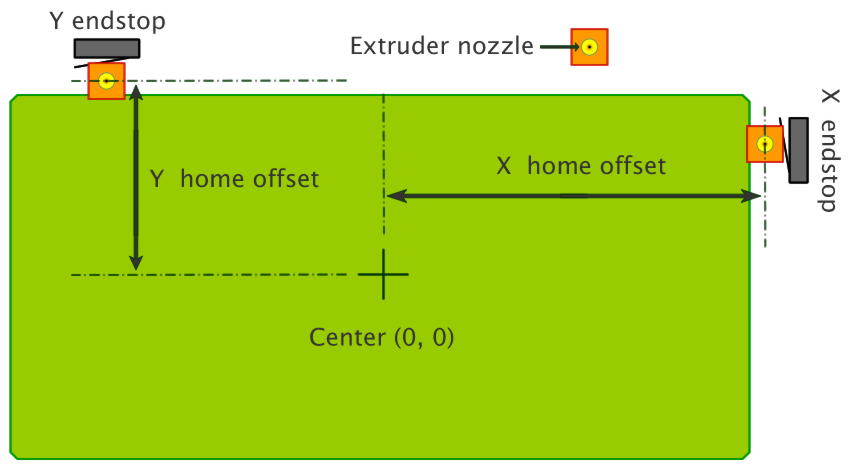
\includegraphics[width=5in]{home-offsets}
    \else
       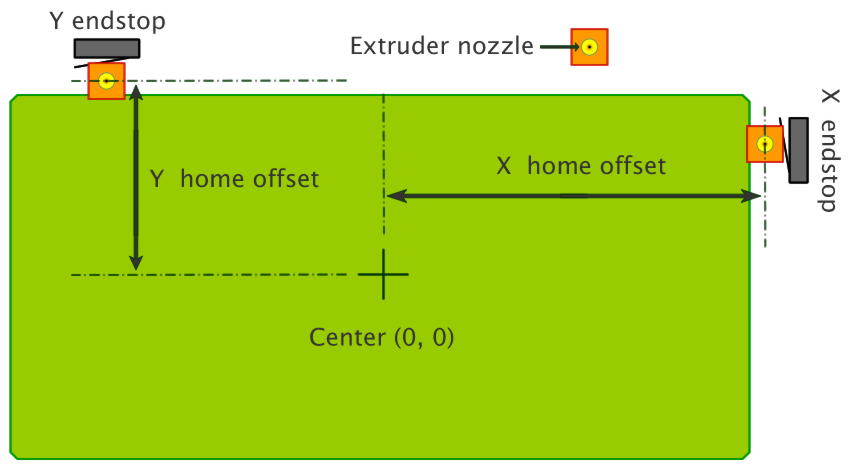
\includegraphics[width=7in]{home-offsets}
    \fi
    \caption{Relationship between the build plate's center and the X \& Y home offsets}
  \label{fig:xy-home-offsets}
\end{figure}

Similarly, the X and Y home offsets tell the printer how far the endstops are from the center of the build platform, giving your printer a general ``sense'' of where it is so that it is able to accurately find the center of the build platform.   This relationship is depicted in  Figure~\ref{fig:xy-home-offsets}. This is important as the printer does not have sensors that tell it where the extruder or build platform are located.  When it begins a print, the printer ``homes'' the axes --- it moves the extruder along the X and Y axes until it hits the endstops and then it raises the platform along the Z axis until reaching that endstop.  Since the resulting position is well-defined, your printer tracks the movement of the plate and extruder so that it always ``knows'' where they are.  As this information is lost whenever you power cycle the printer, homing is a necessity at the start of every print.

The home offsets may be set from the printer's front panel as explained in Section~\ref{sec:homeoff}.  They may also be set from ReplicatorG, MakerWare, and MakerBot Desktop using the ``Machine'' and ``MakerBots'' menus and accessing the onboard parameters.

As most \glspl{slicer} center a print, if your prints do not appear well-centered then your home offsets are likely incorrect because they effectively define (0,0,0) for your printer.   To change the X offset, it is important to note that the X endstop is to the right of the center.  So, if prints are centered too far to the left, you should reduce the X home offset value.  Likewise, if the print is centered too far to the right, then increase the value.  If the prints are centered too far forward then decrease the value of the Y home offset; if the center needs to be moved forward, then increase the value.  Consult Table~\ref{tab:default-offsets} for a list of the default home offsets for many printers.  Note that Cupcakes and Thing-o-Matics do not have default values for their home offsets.  Owners of those two printers set their home offsets by running a calibration script such as that supplied with ReplicatorG.

\begin{bclogo}[logo=\bcinfo, noborder=true, couleurBarre=yellow]{Note}
If you have a dual extruder setup and printing with the left extruder seems off, then the problem is likely in the toolhead offsets, which are described in Section~\ref{sec:toolheadoffsets}.
\end{bclogo}

More care is needed in changing the Z home offset; if made too large, the nozzle and build plate can sustain damage.  Since the Z home offset describes the position of the nozzle in relation to the build plate after homing, increasing the offset tells the printer that the plate is farther from the nozzle than it might actually be.  For example, if you change the home offset value to 1.00~mm and the print begins at 0.15~mm (which is typical for models sliced at 0.30~mm layer height) then the printer will move the build plate up 0.85~mm.  Which, if the build plate was actually closer to the nozzle, can drive the plate into the nozzle.  For this reason, understanding, forethought, and planning are much more important in changing the Z offset value than the X and Y values.  A deeper discussion of the Z home offset may be found in Section~\ref{sec:z-home-offset}.

Note that you should be cautious and thoughtful in changing the Z home offset.  Nevertheless, here are two situations in which you may wish to change the Z home offset: if you have adhesion problems with the first layer of your print, then you may set the Z home offset to a value such as 0.05~mm, making the first layer of the print start 0.05~mm closer to the build plate than it would have otherwise; or, if the extruder is clicking a lot on the first layer since the nozzle is too close to the platform and the filament cannot exit it, then you might decrease the Z home offset to a value such as -0.03~mm.
\index{Home offsets|)}
\index{Offsets!Home|)}
\index{Parameters!Home offsets|)}

\NextFile{parameters-toolhead-offsets.html}

\section{Toolhead Offsets} \label{sec:toolheadoffsets}
\index{Toolhead offsets|(}
\index{Offsets!Toolhead|(}
\index{Parameters!Toolhead offsets|(}

The \glspl{toolhead offset} are only relevant to printers with two extruders.  If your printer has a single extruder setup, then ignore this section.

When, however, you have two extruders, the printer must know the spacing between the nozzles.  The reason being that, when the printer switches extruders, it needs to know what distance to move the extruder carriage so that, for example, the left extruder is now over the exact position at which the right extruder finished printing.  This spacing along the X and Y axes is known as the X and Y toolhead offsets.  It is assumed that the two nozzles are at the same Z position, and thus there is no Z toolhead offset.  Each printer manufacturer has an ``ideal'' set of nozzle spacings, which are built into each printer-specific version of Sailfish.  However, owing to manufacturing tolerances, your nozzles may not quite be spaced with the ideal offsets.  As differences of tenths of millimeters can impact the final appearance of your prints, you can adjust the toolhead offsets to match your printer.

These values may be set from the printer's front panel as explained in Section~\ref{sec:tooloff}.  They may also be set from ReplicatorG, MakerWare, and MakerBot Desktop using the ``Machine'' menus and accessing the onboard parameters.  However, there is a simpler method to set the toolhead offsets: print a calibration print.  Complete step-by-step directions may be found in Section~\ref{sec:dual-calib}.

Additional details on the implementation of toolhead offsets are given in Section~\ref{sec:toolhead-offsets-detail}.  Look to that section if you plan on making your own calibration prints and need to know, for instance, the sign conventions associated with application of the offsets.
\index{Toolhead offsets|)}
\index{Offsets!Toolhead|)}
\index{Parameters!Toolhead offsets|)}

\NextFile{parameters-acceleration.html}

\section{Acceleration}
\index{Acceleration|(}

The print files for any print include directions that determine the speed at which each line segment is printed.  As such, different portions of the print may print at different speeds, causing the printer to speed up or slow down as it transitions between speeds.  By default, when a change of speed is required, the printer effects the change by carefully accelerating to higher speeds or decelerating to lower speeds.  It is possible to turn off this feature by setting the acceleration parameter to ``off'' (Section \ref{sec:acceleration-enable}).  There is no practical reason to do this as printing with acceleration enabled --- the default --- results in smoother, quieter prints that obtain higher speeds.  Turning off acceleration when executing commands at speeds in excess of 30--40~mm/s may cause damage to your printer.
\index{Acceleration|)}

\NextFile{parameters-maximum-accelerations.html}

\subsection{Maximum Accelerations} \label{sec:maxaccels}
\index{Parameters!Maximum acceleration|(}

When acceleration is enabled, your printer needs to pick rates at which to accelerate or decelerate when transitioning between the commanded speeds in a print file.  The maximum acceleration parameters limit how quickly the transition can occur on each axis: X, Y, Z, A, and B.  Note that the A and B axes are the right and left extruders --- if you have only one extruder, then there is no B axis.

The maximum for an axis limits both the acceleration and deceleration with one value that is used for \emph{both}.  The default maximum acceleration values are listed in Table~\ref{tab:def-params}.

If your prints show noticeable overshoot at, say, 90\textdegree\ corners in cubes, then it may well be that your printer is attempting to decelerate faster than its mechanics actually allow.  \index{Print defects!Corner overshoot}The printer has no idea how fast it can really accelerate or decelerate --- it has no built-in feedback system to tell it when it overshoots.  As such, specific printers may need to have their maximum acceleration values changed.  For example, the defaults use the same value for both the X and Y axes.  But, in practice, many printers move far more mass around on their Y axis than their X axis.  With the added mass, the Y axis may not be able to accelerate or decelerate as fast as the X axis can.  Therefore, the maximum acceleration for the Y axis probably should not be the same as that for the X.\footnote{If you see overshoot at corners, it may also be a sign that you need to tune the JKN Advance parameters K or K2.  If the overshoot occurs even at moderate speeds, then see Chapter~\ref{chap:tuning}.}
\index{Parameters!Maximum acceleration|)}

\NextFile{parameters-maximum-speed-changes.html}

\subsection{Maximum Speed Changes} \label{sec:maxspeedchanges}
\index{Parameters!Maximum speed changes|(}

The maximum speed changes regulate the maximum instantaneous changes in speed the printer may effect in transitioning between speeds without carefully accelerating or decelerating through intermediate speeds.  This upper limit is imposed by the maximum X, Y, Z, A, and B speed changes as expressed in units of mm/s.  Note that, while high values can increase printer vibration and even cause it to jerk about, excessively low values significantly increase print times.  Refer to Table~\ref{tab:def-params} for a list of the default maximum speed changes.
\index{Parameters!Maximum speed changes|)}

\NextFile{parameters-auto-leveling.html}

\section{Auto-leveling} \label{sec:alevel-params}
\index{Parameters!Auto-leveling|(}

Some printers incorporate Z-probe mechanisms to measure the build plate position and automatically compensate the print level.  This is referred to as auto-leveling; support for it was introduced in Sailfish~7.7 and 4.7.  This support includes two firmware parameters.  The first, ``auto-level variance'' (Section \ref{sec:alevel-variance}) specifies just how out-of-level your build plate can be and still use auto-leveling.  If the difference in Z height between any two of the three probe points exceeds the variance parameter, then the print is cancelled and you are asked to manually relevel the build plate.\footnote{While the firmware could accommodate a very out-of-level build plate, there is little practical purpose to this.  Sailfish imposes a variance limit as this allows the use of an optimized algorithm for improved print speed.  While some firmwares do allow unlimited variance, this creates significant performance degradation regardless of how level the plate actually is.}  By default, this parameter is set to 0.5~mm.  Its permitted range is anywhere from 0.01~mm to 0.99~mm.  Note, however, that higher values may result in noticeable skew for taller prints if the build plate is uneven.

The second auto-leveling related parameter is the maximum number of probe hits which will be tolerated before the printer pauses and requests manual intervention (Section~\ref{sec:alevel-maxhits}). Set this parameter to the value 0 to ignore all probe hits once the print begins.  Otherwise, it may be set to any value in the range 1 -- 200.  The default value is 20, meaning that, on probe hit number 21, the printer pauses.  The count of hits is reset back to 0 after resuming the print.
\index{Parameters!Auto-leveling|)}

\NextFile{parameters-deprime.html}

\section{Firmware Retraction (Deprime)} \label{sec:deprime}
\index{Deprime}
\index{Deprime!On travel}
\index{Retraction, firmware}
\index{Parameters!Deprime|(}

This allows you to configure the printer with a filament retraction setting (in units of steps) to be used when pauses occur, planned or otherwise.  You are able to separately control the right extruder, A, and the left extruder, B.  If your printer is only equipped with one extruder, it is considered ``A''.

When a deprime setting is non-zero, the printer will deprime the associated extruder by the specified number of steps when it is active and any of the following occurs:

\begin{enumerate}
\item Pausing, whether user initiated or a P-Stop generated pause.
\item When the printing process is temporarily idle because the queue of processed segments has run out.  Depriming the active extruder will help prevent blemishes.
\item If ``Deprime on Travel'' is enabled, then, when the printer detects a \gls{travel move} it will deprime.  However, it is difficult for the printer to truly detect this, as the printing of very low layer heights may require many short printing moves which are not accompanied by extrusion.  In actuality, the printer can only identify travel moves if the print commands disable the extruder stepper motor before effecting a move.  Note that most slicers \emph{do not} disable the extruders before a travel move, as it may allow the filament to back out of the extruder by an unknown amount.
\end{enumerate}

When printing resumes, the printer then feeds the filament back in by the same number of steps by which it was deprimed.

By default ``Deprime on Travel'' is disabled, though deprime is set to a non-zero value for each extruder as per Table~\ref{tab:def-params}.
\index{Parameters!Deprime|)}

\NextFile{parameters-slowdown.html}

\section{Slowdown} \label{sec:slowdown}
\index{Parameters!Slowdown|(}

By default, this feature is enabled.  It makes the printer slow down when the queue of already processed line segments is running low.  By printing the remaining queued segments more slowly, there is more time for the queue to refill.  This helps prevent the printer sitting idle when the queue completely empties, eliminating the tiny blemishes that may form while plastic continues to ooze from the idle extruder.

Normally, the queue of processed line segments is full.  There are only two common situations in which the queue starts to run dry: first, when quickly printing many short line segments in small, fine detail;  second, when printing over a serial USB connection where the computer sending the data over the USB is slow.

There is no practical reason to disable this option other than to see the effects of printing small fine detail quickly (120~mm/s) without it enabled.
\index{Parameters!Slowdown|)}

\NextFile{parameters-rgb-led.html}

\section{Lighting (RGB LED)} \label{sec:rgb-led}
\index{RGB LED lighting}
\index{Lighting}
\index{Parameters!RGB LED|(}

Some printers come equipped with RGB LED lighting strips to light the printing bay.  The printer controls this lighting, and sets the colors which appear.  The settings for these lighting strips may only be controlled from your computer, most comfortably from ReplicatorG's ``Onboard Preferences'' window, accessed from its ``Machine'' menu.  MakerWare and Desktop may also be used, but not as conveniently.

Three aspects of the lighting may be controlled:

\begin{enumerate}
\item The choice of color: white (0), red (1), orange (2), pink (3), green (4), blue (5), purple (6), off (7), and custom (8).  The default selection is white. Use ``off'' (7) to turn the lighting off.  When using MakerWare or Desktop, you will need to use the listed numeric values with the ``Basic Color'' setting.
\item A custom color will be used when you set the color choice to ``custom'' (8).  When using ReplicatorG, a ``color picker'' allows selection of a color from a palette.  From MakerWare and Desktop, you must provide an RGB value as three integers, each in the range 0 -- 255.
\item You can elect to have the lighting cycle from blue (cool) to red (hot) as each heater heats up.  Once heating is complete and the printer begins printing, the lighting switches back to the normal color choice that has been set (or white if none has been set). In MakerWare and Desktop this appears as the option ``Led Heat''.  In ReplicatorG, this is the ``show heating progress by changing the lighting color'' checkbox.
\end{enumerate}
\index{Parameters!RGB LED|)}
